% !TEX TS-program = xelatex
% !BIB TS-program = bibtex
\documentclass[12pt,letterpaper]{article}
\usepackage{style/dsc180reportstyle}
\usepackage{tikz}
\usepackage{pgfplots}
\pgfplotsset{compat=1.18}

\title{Differentially private synthetic data generation via DP-VAE}

\author{Mehak Kapur \\
  {\tt mekapur@ucsd.edu} \\\And
  Hana Tjendrawasi  \\
  {\tt htjendrawasi@ucsd.edu} \\\And
  Jason Tran \\
  {\tt jat037@ucsd.edu} \\\And
  Phuc Tran \\
  {\tt pct001@ucsd.edu} \\\And
  Yu-Xiang Wang \\
  {\tt yuxiangw@ucsd.edu} \\}

\begin{document}
\maketitle

\begin{abstract}
    Differentially private synthetic data generation enables the release of realistic datasets while rigorously protecting the privacy of individuals in the source data. We implement a differentially private variational autoencoder (DP-VAE) trained using differentially private stochastic gradient descent (DP-SGD), which privatizes model training through per-sample gradient clipping and calibrated Gaussian noise injection. Applying this approach to a realistic telemetry dataset, we demonstrate that DP-VAE successfully generates high-fidelity synthetic records under a modest privacy budget ($\varepsilon = 4.0$). Our evaluation shows that categorical distributions are preserved within $8\%$ absolute deviation, and downstream classification models trained on synthetic data achieve accuracy comparable to those trained on real data.
\end{abstract}

\begin{center}
Code: \url{https://github.com/jktrns/dsc-180a-q1}
\end{center}

\maketoc
\clearpage

\section{Introduction}

\subsection{Motivation and problem statement}

Contemporary machine learning requires large, richly annotated datasets that frequently encode sensitive personal information. The utility of such data for scientific and commercial progress stands in tension with the imperative to protect individual privacy. Traditional anonymization techniques (e.g., removal of explicit identifiers, aggregation) have proven inadequate against adversaries with auxiliary information. \textit{Differential privacy} (DP) provides a rigorous mathematical framework for this challenge, ensuring that any individual's participation in a dataset has negligible impact on the algorithm's output distribution.

The promise of differential privacy is quantified by a \textit{privacy budget} $\varepsilon$, where smaller values confer stronger privacy guarantees at the cost of reduced data utility. Thus, we have a trade-off that pervades all differentially private mechanisms; perfect privacy ($\varepsilon = 0$) is achieved only by revealing nothing whatsoever, yet an unbounded $\varepsilon$ will permit arbitrary disclosure. We must operate within a regime of small but non-trivial $\varepsilon$ to manage this trade-off.

\textit{Synthetic data generation} under differential privacy is particularly appealing here. In this setting, the curator (a trusted party) releases an entirely artificial dataset that captures the statistical properties of the original data while satisfying formal privacy guarantees. Such synthetic datasets come with the benefit of being analyzable using conventional statistical software. Moreover, once released, synthetic data imposes no ongoing privacy cost, unlike interactive mechanisms where privacy loss accumulates with each query.

\textit{Differentially private stochastic gradient descent} (DP-SGD) \citep{abadi2016deep} provides a principled approach to training generative models under formal privacy guarantees. By clipping per-sample gradients and injecting calibrated Gaussian noise at each optimization step, DP-SGD bounds the influence any single training example can exert on the learned model parameters. We apply DP-SGD to train a variational autoencoder (VAE) on tabular telemetry data, investigating the privacy-utility trade-off and evaluating the fidelity of the resulting synthetic dataset.

\newpage

\subsection{Prior work}

DP, introduced by \citet{dwork2014algorithmic}, promises that the behavior of an algorithm is approximately invariant to the inclusion or exclusion of any single individual's data. This promise is formalized through the requirement that \textit{neighboring databases} (those differing by precisely one record) yield indistinguishable output distributions, up to a multiplicative factor $\exp(\varepsilon)$ and additive slack $\delta$. The seminal work established key mechanisms (e.g., the Laplace and Gaussian mechanisms for numeric queries), along with composition theorems demonstrating that privacy loss accumulates across multiple analyses.

The extension of differential privacy to deep learning proved non-trivial. \citet{abadi2016deep} developed DP-SGD by recognizing that standard gradient descent leaks information through the unbounded influence any single training example can exert on model parameters. Their solution bounds this influence through gradient clipping while injecting calibrated Gaussian noise to mask the contribution of individual samples. Critically, they introduced the \textit{moments accountant}, a privacy accounting technique that yields substantially tighter bounds on cumulative privacy loss than naive composition would suggest.

Building upon DP-SGD, researchers have applied differentially private optimization to various generative architectures. \citet{ghalebikesabi2023differentially} demonstrated that fine-tuning diffusion models with DP-SGD generates high-fidelity synthetic images, though their approach requires substantial privacy budgets ($\varepsilon \approx 32$ for CIFAR-10). Variational autoencoders (VAEs) present an attractive alternative for tabular data, as their latent-space structure naturally regularizes generation, and their relatively compact architectures reduce the number of noisy gradient updates required to converge. We leverage these properties by training a DP-VAE, combining DP-SGD with the flexibility of variational inference.

% \newpage

% \section{Background}

% We represent databases as histograms $x \in \mathbb{N}^{|\mathcal{X}|}$ over a universe $\mathcal{X}$ of record types, where $x_i$ denotes the count of records of type $i \in \mathcal{X}$ (e.g., $\mathcal{X} = \{\text{student},\, \text{instructor},\, \text{staff}\}$, $x = (150, 30, 20)$). Two databases are \textit{neighboring} if they differ in the record count of exactly one individual (i.e., their $\ell_1$ distance is at most 1: $\|x - y\|_1 \leq 1$).

% A randomized mechanism $\mathcal{M} \colon \mathbb{N}^{|\mathcal{X}|} \rightarrow \Delta(B)$ maps databases to probability distributions over outputs in range $B$, where $\Delta(B)$ denotes the \textit{probability simplex} (i.e., the set of all probability distributions over $B$).

% \begin{definition}[Differential privacy \citep{dwork2014algorithmic}]
% \label{def:dp}
% $\mathcal{M}$ satisfies $(\varepsilon, \delta)$-differential privacy if for all neighboring databases $x, y$ with $\|x - y\|_1 \leq 1$ and all measurable sets $S \subseteq B$:
% \begin{equation}
% \Pr[\mathcal{M}(x) \in S] \leq \exp(\varepsilon) \Pr[\mathcal{M}(y) \in S] + \delta
% \end{equation}
% When $\delta = 0$, we say $\mathcal{M}$ is $\varepsilon$-differentially private.
% \end{definition}

% For small $\varepsilon$, the bound $\exp(\varepsilon) \approx 1 + \varepsilon$ ensures outputs are nearly equally likely regardless of any individual's participation. The slack $\delta$ permits rare catastrophes; we conventionally require $\delta \ll 1/\|x\|_1$.

% TODO

\newpage

\section{Methods}

\subsection{Data}

Our experiments center on a 152{,}356-row telemetry table that mimics privacy-critical product instrumentation. Each record contains a product family label (\textbf{A--F or Others}), an event label (\textbf{open}, \textbf{close}, \textbf{save}, \textbf{reset}, \textbf{error}), and a timestamp between May and July 2024. Although the table is synthetic, we treat it as sensitive and apply all processing steps exactly as we would for proprietary logs. Pre-training, we drop the anonymized user identifier, convert timestamps to Unix seconds, one-hot encode the categorical columns, and z-score the time feature using a \texttt{ColumnTransformer}. The resulting feature matrix has 13 dimensions, with 12 categorical indicators plus one standardized numeric attribute.

\subsection{DP-VAE generator}
We train a \textit{differentially private variational autoencoder} (DP-VAE) to learn a generative model of the telemetry distribution. The encoder maps our 13-dimensional inputs to a 128-unit hidden layer and outputs a 16-dimensional mean and log-variance. The decoder mirrors this structure and produces logits for each categorical attribute, plus a numeric head for the standardized timestamp. DP-SGD is applied for up to 30 epochs using a batch size of $256$, clip norm $1.0$, noise multiplier $1.0$, and learning rate $3 \times 10^{-3}$. Training halts either after completing all epochs or once the privacy budget is consumed ($\varepsilon = 4.0$ at $\delta = 10^{-5}$). Training minimizes the sum of categorical cross-entropies, mean-squared error for the numeric column, and the Kullback--Leibler divergence between the inferred posterior and the unit Gaussian prior. After training, we sample $z \sim \mathcal{N}(0, I)$, decode to logits, take argmaxes for the categories, and invert the timestamp scaler before clipping to the observed range.

% \begin{table}[H]
% \centering
% \begin{tabular}{lc}
% \toprule
% \textbf{Hyperparameter} & \textbf{Value} \\
% \midrule
% Architecture & 13-128-128 encoder, mean/logvar heads, symmetric decoder \\
% Batch size & 256 \\
% Learning rate & $3 \times 10^{-3}$ (Adam) \\
% Noise multiplier & 1.0 \\
% Epoch budget & 30 (with early stopping once $\varepsilon \geq 3.9$) \\
% Latent dimension & 16 \\
% Clip norm & 1.0 \\
% \bottomrule
% \end{tabular}
% \caption{Differentially private VAE training configuration.}
% \end{table}

\begin{algorithm}[h]
\caption{Differentially private VAE training}
\label{alg:dpvae}
\SetKwInOut{KwInput}{Input}
\SetKwInOut{KwOutput}{Output}
\KwInput{Dataset $D$, noise multiplier $\sigma$, clip norm $C$, target $\varepsilon^\star$}
\KwOutput{Trained parameters $\theta$ and privacy accountant state}
$\varepsilon \gets 0$\;
\While{$\varepsilon < \varepsilon^\star$}{
    Sample batch $B \subset D$\;
    Compute reconstruction loss
    $\mathcal{L}_{\text{rec}} = \mathrm{CE}(x_{\text{cat}}, \hat{x}_{\text{cat}}) + \mathrm{MSE}(x_{\text{time}}, \hat{x}_{\text{time}})$\;
    Compute KL term $\mathcal{L}_{\text{kl}} = \mathrm{KL}(q_\theta(z|x) \parallel \mathcal{N}(0, I))$\;
    $\mathcal{L} \gets \mathcal{L}_{\text{rec}} + \mathcal{L}_{\text{kl}}$\;
    Clip per-example gradients of $\mathcal{L}$ to norm $C$\;
    Add Gaussian noise with standard deviation $\sigma C$ and apply Adam update\;
    $\varepsilon \gets \texttt{AccountantUpdate}(\varepsilon)$\;
}
\end{algorithm}

\newpage

\section{Evaluation}
All measurements reported below come from \texttt{notebooks/03-validation.ipynb}, which consumes only the released synthetic dataset for analysis.

\subsection{Marginal distributions}
We compare empirical distributions for every categorical column. Product family proportions differ by at most $3.95\%$ absolute (class \textbf{B}), while event label deltas remain below $7.4\%$ (class \textbf{close}). Table~\ref{tab:combined-dist} and Figure~\ref{fig:combined-bar} detail these marginals.

\begin{table}[H]
\centering
\begin{tabular}{lcccc|lcccc}
\toprule
\multicolumn{5}{c|}{\textbf{Product type}} & \multicolumn{5}{c}{\textbf{Event type}} \\
\textbf{Class} & \textbf{Real} & \textbf{Synthetic} & \textbf{$|\Delta|$} & \textbf{$|\Delta|$\%} &
\textbf{Class} & \textbf{Real} & \textbf{Synthetic} & \textbf{$|\Delta|$} & \textbf{$|\Delta|$\%} \\
\midrule
A & 0.152 & 0.153 & 0.001 & 0.09 & close & 0.308 & 0.381 & 0.074 & 7.4 \\
B & 0.252 & 0.291 & 0.040 & 4.0 & error & 0.032 & 0.011 & 0.022 & 2.2 \\
C & 0.187 & 0.197 & 0.010 & 1.0 & open & 0.383 & 0.427 & 0.044 & 4.4 \\
D & 0.200 & 0.229 & 0.028 & 2.8 & reset & 0.068 & 0.018 & 0.050 & 5.0 \\
E & 0.010 & 0.000 & 0.010 & 1.0 & save & 0.210 & 0.163 & 0.047 & 4.7 \\
F & 0.099 & 0.046 & 0.053 & 5.3 & & & & & \\
Others & 0.100 & 0.085 & 0.016 & 1.6 & & & & & \\
\bottomrule
\end{tabular}
\caption{Distributional comparison for product type and event type}
\label{tab:combined-dist}
\end{table}

\begin{figure}[H]
\centering
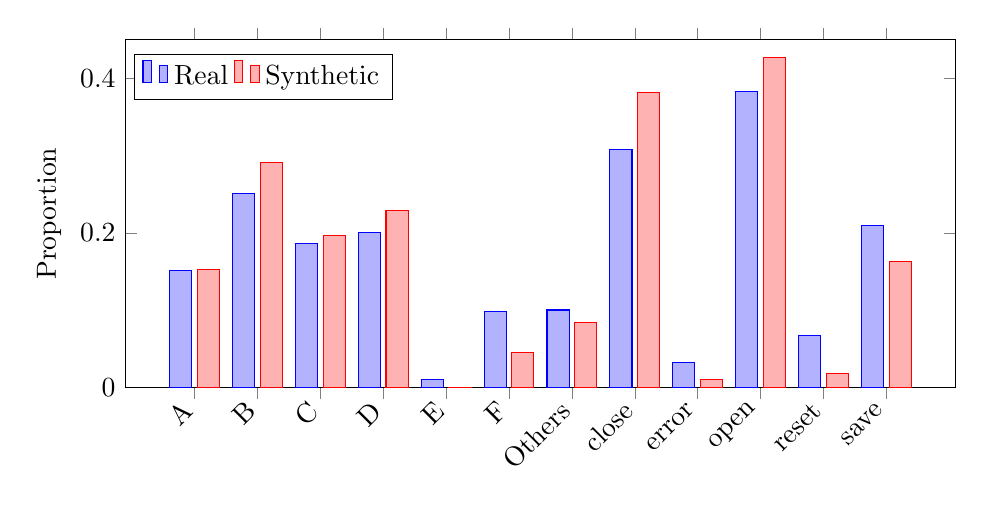
\begin{tikzpicture}
\begin{axis}[
    ybar,
    bar width=8pt,
    width=\linewidth,
    height=6cm,
    ylabel={Proportion},
    symbolic x coords={A,B,C,D,E,F,Others,close,error,open,reset,save},
    xtick=data,
    xtick style={font=\scriptsize},
    legend style={at={(0.5,-0.35)},anchor=north,legend columns=-1},
    ymin=0,
    ymax=0.45,
    legend style={
        at={(0.01,0.96)},
        anchor=north west
    },
    x tick label style={rotate=45,anchor=east},
]
\addplot coordinates {(A,0.1516) (B,0.2515) (C,0.1869) (D,0.2004) (E,0.0104) (F,0.0989) (Others,0.1004)
(close,0.3077) (error,0.0323) (open,0.3827) (reset,0.0675) (save,0.2098)};
\addplot coordinates {(A,0.1525) (B,0.2910) (C,0.1971) (D,0.2287) (E,0.0001) (F,0.0459) (Others,0.0847)
(close,0.3813) (error,0.0107) (open,0.4269) (reset,0.0180) (save,0.1631)};
\legend{Real, Synthetic}
\end{axis}
\end{tikzpicture}
\caption{Product-type and event-type distributions}
\label{fig:combined-bar}
\end{figure}

\newpage

\subsection{Timestamp distribution}
Kernel density plots over \texttt{TimeSeconds} reveal a slight smoothing effect in the synthetic timeline; the Kolmogorov--Smirnov statistic is $0.137$ with $p < 10^{-150}$ (see Figure~\ref{fig:timeseconds-kde}).

\begin{figure}[H]
\centering
\begin{tikzpicture}
\begin{axis}[
    width=\linewidth,
    height=6cm,
    xlabel={Timestamp (seconds)},
    ylabel={Density},
    ymin=0,
    legend style={
        at={(0.99,0.96)},
        anchor=north east
    },
    grid=both,
    minor grid style={gray!20},
    major grid style={gray!40},
]
    \addplot+[smooth, color=RoyalBlue]
        table [x=seconds, y=density, col sep=comma] {figure/kde-real.csv};
    \addlegendentry{Real}
    \addplot+[smooth, color=BrickRed]
        table [x=seconds, y=density, col sep=comma] {figure/kde-synthetic.csv};
    \addlegendentry{Synthetic}
\end{axis}
\end{tikzpicture}
\caption{Kernel density estimate of \texttt{TimeSeconds}}
\label{fig:timeseconds-kde}
\end{figure}

Figure~\ref{fig:timeseconds-kde} highlights that the DP-VAE concentrates probability mass nearer the middle of the observation window. The synthetic timestamps average $2.77\times 10^{4}$ seconds (7.7 hours) earlier and exhibit $27\%$ less variance than the real data, even while sharing the same support. Table~\ref{tab:time-moments} reports that despite the statistically significant gap, both means remain within half a standard deviation of each other, explaining why downstream accuracy barely changes.

\begin{table}[H]
\centering
\begin{tabular}{lcccc}
\toprule
\textbf{Metric} & \textbf{Real} & \textbf{Synthetic} & \textbf{$|\Delta|$} & \textbf{$|\Delta|$\%} \\
\midrule
Mean & $1\,718\,462\,125.60$ & $1\,718\,434\,451.10$ & $27\,674.50$ & $0.0016$ \\
Standard deviation & $2\,265\,577.72$ & $1\,646\,876.40$ & $618\,701.32$ & $27.31$ \\
Minimum & $1\,714\,521\,637.00$ & $1\,714\,521\,637.00$ & $0.00$ & $0.00$ \\
Maximum & $1\,722\,383\,984.00$ & $1\,722\,383\,984.00$ & $0.00$ & $0.00$ \\
\bottomrule
\end{tabular}
\caption{Descriptive statistics for \texttt{TimeSeconds} (unit: seconds)}
\label{tab:time-moments}
\end{table}

\subsection{Downstream classification}
To assess downstream utility, we train multinomial logistic regressions using product family and timestamp as predictors. Training on synthetic data and evaluating on the untouched telemetry table attains $0.380$ accuracy, essentially matching the real-only baseline of $0.381$. The per-class report in Table~\ref{tab:classification-report} shows that both models struggle on the rare \textbf{error}, \textbf{reset}, and \textbf{save} events, predicting none of them with the current feature set. Synthetic training offers a recall boost on the dominant \textbf{close} class (0.418 vs.\ 0.195) while the baseline maintains higher recall for \textbf{open} events. Macro and weighted averages remain nearly identical.

\begin{table}[H]
\centering
\begin{tabular}{lcccc|cccc}
\toprule
& \multicolumn{4}{c|}{\textbf{Synthetic training ($\text{syn}\rightarrow\text{real}$)}} & \multicolumn{4}{c}{\textbf{Baseline ($\text{real}\rightarrow\text{real}$)}} \\
\textbf{Class} & \textbf{Precision} & \textbf{Recall} & \textbf{F1} & \textbf{Support} & \textbf{Precision} & \textbf{Recall} & \textbf{F1} & \textbf{Support} \\
\midrule
close & 0.321 & 0.418 & 0.363 & 46{,}885 & 0.343 & 0.195 & 0.249 & 14{,}020 \\
error & 0.000 & 0.000 & 0.000 & 4{,}925 & 0.000 & 0.000 & 0.000 & 1{,}461 \\
open & 0.418 & 0.656 & 0.511 & 58{,}306 & 0.389 & 0.837 & 0.531 & 17{,}544 \\
reset & 0.000 & 0.000 & 0.000 & 10{,}277 & 0.000 & 0.000 & 0.000 & 3{,}033 \\
save & 0.000 & 0.000 & 0.000 & 31{,}963 & 0.000 & 0.000 & 0.000 & 9{,}649 \\
\midrule
accuracy & \multicolumn{4}{c|}{0.380} & \multicolumn{4}{c}{0.381} \\
macro avg & 0.148 & 0.215 & 0.175 & 152{,}356 & 0.146 & 0.206 & 0.156 & 45{,}707 \\
weighted avg & 0.259 & 0.380 & 0.307 & 152{,}356 & 0.255 & 0.381 & 0.280 & 45{,}707 \\
\bottomrule
\end{tabular}
\caption{Per-class metrics for multinomial logistic regression}
\label{tab:classification-report}
\end{table}

\subsection{Error rate z-scores}
We evaluate whether the synthetic data preserves the ability to identify product types with above-average error rates. For each product type $P$, we compute the error rate $\text{ErrorRate}_P = \text{ErrorCount}_P / \text{TotalCount}_P$ and its z-score across all products. Products with $Z > 0$ represent those with above-average error rates. Table~\ref{tab:zscore-comparison} and Figure~\ref{fig:zscore-bar} compare these statistics between real and synthetic data, while we report $L_\infty$ error (maximum absolute z-score deviation) and IOU (intersection over union of the ``top sets'' with $Z > 0$) as aggregate metrics.

\begin{table}[H]
\centering
\begin{tabular}{lcccc}
\toprule
\textbf{Product} & \textbf{Real error rate} & \textbf{Synthetic error rate} & \textbf{Real $Z$} & \textbf{Synthetic $Z$} \\
\midrule
A & 0.0054 & 0.0000 & $-0.91$ & $-0.54$ \\
B & 0.0200 & 0.0021 & $-0.39$ & $-0.40$ \\
C & 0.0014 & 0.0000 & $-1.05$ & $-0.54$ \\
D & 0.0890 & 0.0420 & $+2.06$ & $+2.40$ \\
E & 0.0190 & 0.0000 & $-0.43$ & $-0.54$ \\
F & 0.0510 & 0.0087 & $+0.71$ & $+0.07$ \\
Others & 0.0312 & 0.0012 & $+0.01$ & $-0.46$ \\
\bottomrule
\end{tabular}
\caption{Error rates and z-scores by product type for real vs.\ synthetic data.}
\label{tab:zscore-comparison}
\end{table}

\begin{figure}[H]
\centering
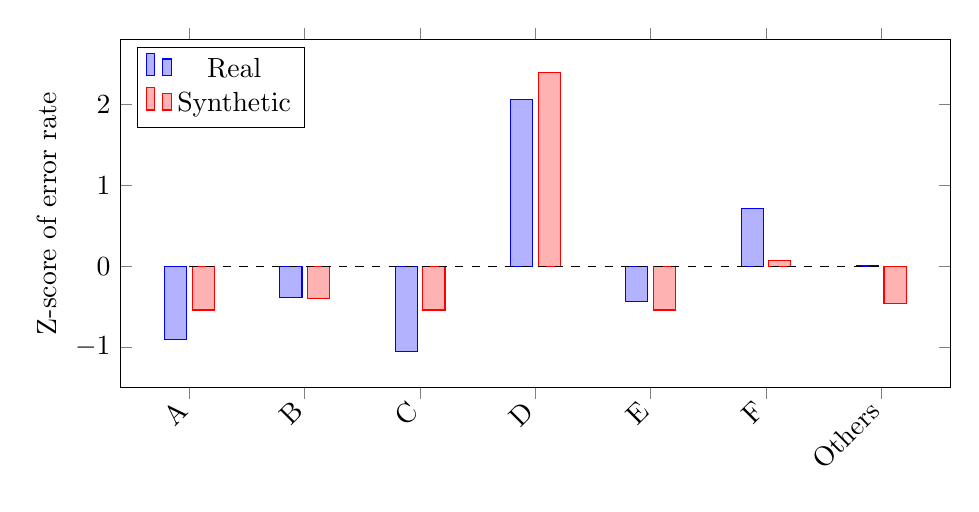
\begin{tikzpicture}
\begin{axis}[
    ybar,
    bar width=8pt,
    width=\linewidth,
    height=6cm,
    ylabel={Z-score of error rate},
    symbolic x coords={A,B,C,D,E,F,Others},
    xtick=data,
    legend style={at={(0.02,0.98)}, anchor=north west},
    ymin=-1.5,
    ymax=2.8,
    x tick label style={rotate=45,anchor=east},
]
\addplot coordinates {(A,-0.91) (B,-0.39) (C,-1.05) (D,2.06) (E,-0.43) (F,0.71) (Others,0.01)};
\addplot coordinates {(A,-0.54) (B,-0.40) (C,-0.54) (D,2.40) (E,-0.54) (F,0.07) (Others,-0.46)};
\legend{Real, Synthetic}
\draw[black, dashed] (axis cs:A,0) -- (axis cs:Others,0);
\end{axis}
\end{tikzpicture}
\caption{Error rate z-scores by product type, where $Z > 0$ indicates above-average error}
\label{fig:zscore-bar}
\end{figure}

The real data identifies \textbf{D}, \textbf{F}, and \textbf{Others} as products with above-average error rates. The synthetic data correctly flags \textbf{D} (the clear outlier with $Z \approx 2.4$) and \textbf{F}, but misses \textbf{Others}, whose real z-score of $0.01$ exists barely above the threshold. This yields an IOU of $0.67$ (2 of 3 products recovered). The $L_\infty$ error of $0.64$ arises primarily from the ``Others'' discrepancy. Despite the under-representation of error events in the synthetic data (1.07\% vs.\ 3.23\%), the DP-VAE preserves the relative ranking of error-prone products, as it correctly identifies \textbf{D} as the dominant source of errors.

\begin{table}[H]
\centering
\begin{tabular}{lc}
\toprule
\textbf{Metric} & \textbf{Value} \\
\midrule
Max product-type delta & $3.95\%$ (class \textbf{B}) \\
Max event-type delta & $7.36\%$ (class \textbf{close}) \\
KS statistic (time) & $0.137$ ($p < 10^{-150}$) \\
LogReg accuracy (syn$\rightarrow$real) & $0.380$ \\
LogReg accuracy (real$\rightarrow$real) & $0.381$ \\
Z-score $L_\infty$ error & $0.64$ \\
Z-score IOU (top set) & $0.67$ \\
\bottomrule
\end{tabular}
\caption{Key validation metrics produced by \texttt{03-validation.ipynb}}
\label{tab:summary-metrics}
\end{table}

\newpage

\section{Conclusion}

We presented a differentially private variational autoencoder trained with DP-SGD for generating synthetic telemetry data under a privacy budget of $\varepsilon = 4.0$. Our evaluation demonstrates that the DP-VAE preserves categorical marginal distributions within $8\%$ absolute deviation, and produces synthetic data on which downstream classifiers achieve accuracy virtually identical to models trained on real data ($0.380$ vs.\ $0.381$).

Primary limitations stem from DP-SGD's inherent bias against rare classes, as gradient clipping and noise injection disproportionately suppress low-frequency modes. This leads to under-representation of minority categories (e.g., product \textbf{E}, event \textbf{error}). Similarly, the timestamp distribution contracts toward the center of the observation window due to continuous features being normalized via noise.

Despite these limitations, the synthetic data correctly identifies the dominant high-error product (\textbf{D}) and preserves the relative ranking of error-prone products, demonstrating practical utility for aggregate analytics. Future work could explore alternative privacy-preserving frameworks to improve fidelity on rare classes while maintaining strong privacy guarantees.

\newpage

\makereference

\nocite{*}
\bibliography{reference}
\bibliographystyle{style/dsc180bibstyle}

\end{document}